\lecture{13}{25. November}{Sandsynlighedsregning}

\section{Den uniforme fordeling (2.3)}
Vi betragter et interval fra $\alpha$ til $\beta$ og vi trækker et helt tilfældigt tal mellem punkterne vil valgene være uniformfordelt.
\begin{definition} [Den uniforme fordeling]
  Lad $\alpha < \beta$. En stokastisk variabel $X$ siges at være uniformfordelt på intervalet $(\alpha; \beta)$, hvis $X$ er kontinuert med tæthed
  \[ 
  f(x) = \frac{1}{\beta - \alpha}, \quad \text{for } \alpha < x < \beta, \quad \text{og } f(x) = 0 \text{ ellers}
  .\]
  Den uniforme fordeling beskriver et helt tilfældigt valg mellem $\alpha$ og $\beta$. Den uniforme fordeling på $(0, 1)$ har tæthed $f$ givet ved $f(x) = \frac{1}{1-0} =1$ for $0 < x <1$, og $f(x) = 0$ ellers.
\end{definition}

\begin{sæt} [Fordelingsfunktionen for den uniforme fordeling]
  Fordelingsfunktionen $F$ for en uniform fordeling på $(\alpha; \beta)$ er givet ved
  \[ 
  F(x) = \frac{x-\alpha}{\beta - \alpha}, \quad \text{for} \quad \alpha \leq x \leq \beta
  .\]
  Det følger af
  \[ 
  F(x) = \int_{-\infty}^{x} f(s) \, \mathrm{d}s = \int_{\alpha}^{x} \frac{1}{\beta - \alpha} \, \mathrm{d}x = \frac{x - \alpha}{\beta - \alpha}
  .\]
\end{sæt}

\begin{sæt} [Middelværdi og Varians for en uniform fordelign]
  Middelværdien $E$ af en uniformfordelt stokastisk variabel $X$ er
  \[ 
    E[X] = \frac{\alpha + \beta}{2}
  .\]
  Dette svarer til midtpunktet af $(\alpha; \beta)$.
  \bigbreak
  Variansen $\mathrm{Var}$ af en uniformfordelt stokastisk variabel $X$ er
  \[ 
  \mathrm{Var}(X) = \frac{\beta - \alpha}{12}
  .\]
  Dette svarer til intervallængden delt med 12.
  \tcblower
  Middelværdien af en stokastisk variabel er generelt givet ved
  \[ 
    E[X] = \int_{-\infty}^{\infty} x f(x) \, \mathrm{d}x 
  .\]
  Vi kan indsætte vores tæthedsfunktion $f(x)$ som
  \begin{align*}
    E[X] &= \int_{\alpha}^{\beta} x \frac{1}{\beta - \alpha} \, \mathrm{d}x \\
    &= \frac{1}{\beta - \alpha} \int_{\alpha}^{\beta} x \\
    &= \frac{1}{\beta - \alpha} \left[ \frac{1}{2}x^2 \right]_{\alpha}^{\beta} \\
    &= \frac{1}{\beta - \alpha} \cdot \frac{1}{2} \beta^2 - \alpha^2 \\
    &= \frac{1}{\beta - \alpha} \cdot \frac{1}{2}(\beta - \alpha)(\beta + \alpha) \\
    &= \frac{\beta + \alpha}{2}
  .\end{align*}
  Altså er det vist.
\end{sæt}

\begin{eks} [Uniformfordeling]
  Lad $X$ være uniformfordelt på $(0, 10)$. Bestem $P(3 < X < 7$.
  \bigbreak
  Vi vil regne dette vha. fordelingsfunktioner. Vi har fordelingsfunktionen som
  \[ 
  F(x) = \frac{x-0}{10 - 0} = \frac{x}{10}
  .\]
  Vi kan nu finde $P(3 < X < 7)$ som tilvæskten i fordelingsfunktionen fra den nedre til den øvre grænse. Vi får altså
  \[ 
  P(3 < X < 7) = \frac{7}{10} - \frac{3}{10} = \frac{2}{5}
  .\]
  Vi kunne også have gjort dette vha. integration af tæthedsfunktionen fra nedre til øvre grænse. som
  \[ 
  \int_{0}^{10} f(x) \, \mathrm{d}x 
  .\]
\end{eks}

\section{Normalfordelingen (2.4)}
Normalfordelingen er en af de vigtigste og hyppigst brugte fordelinger.

\begin{definition} [Normalfordeling]
  Lad $\mu \in \mathbb{R}$ og $\sigma^2 \geq 0$. En stokastisk variabel $X$ siges at være \textit{normalfordelt} med parametre $\mu$ og $\sigma^2$, hvis $X$ har tæthedsfunktion givet ved
  \[ 
  f(x) = \frac{1}{\sqrt{2\pi}\sigma}e^{\frac{(x-\mu)^2}{2\sigma^2}} \quad \text{for alle } x
  .\]
  Hvis $\mu = 0$ og $\sigma^2 = 1$ siges $X$ endvidere at være standard-normalfordelt.
\end{definition}

\begin{sæt} [Middelværdien og variansen for normalfordelingen]
  Lad $X$ være normalfordelt med parametre $\left(\mu, \sigma^2\right)$ så gælder at
  \begin{align*}
    E[X] &= \mu \\
    \mathrm{Var}(X) &= \sigma^2
  .\end{align*}
\end{sæt}

\begin{sæt} [Fordelingsfunktionen for standard-normalfordelingen]
  Fordelingsfunktionen for standard-norrmalfordelingen skrives som
  \[ 
  \Phi(x) = \frac{1}{\sqrt{2\pi}} \int_{-\infty}^{x} e^{-\frac{s^2}{2}} \, \mathrm{d}s
  .\]
  Dette integrale kan imidlertid ikke løses analytisk og man er derfor nødt til at have gang i sin lommeregner eller finde en tabel (som \autoref{fig:F13_1}) og slå op i.
\end{sæt}

\subsection{Tabel over værdier af fordelingsfunktionen for standard-normalfordelingen}
\begin{figure} [ht]
  \centering
  \caption{Tabel over værdien af $\Phi(x)$ for forskellige $x$ for standard-normalfordelingen.}
  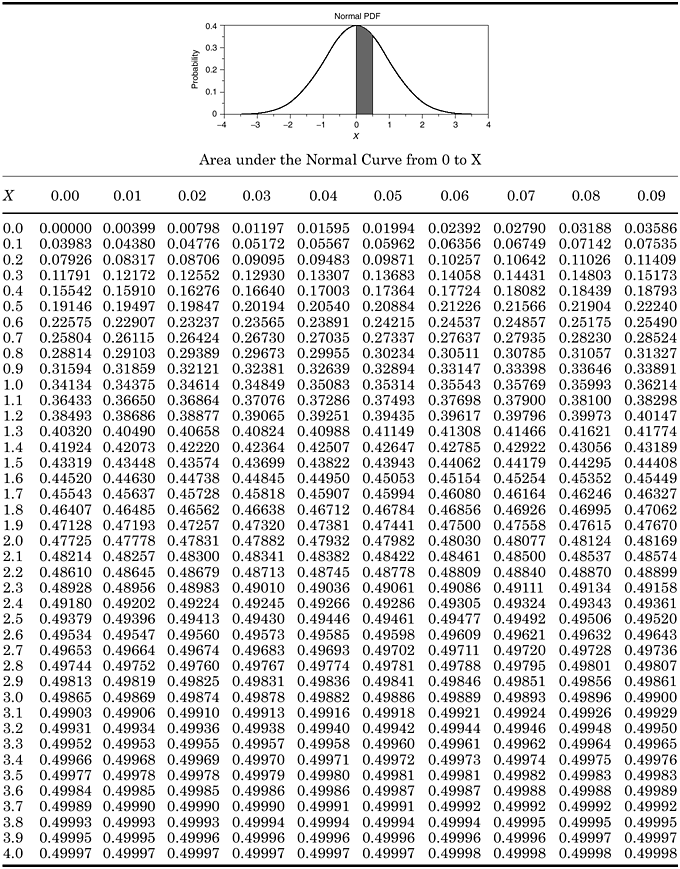
\includegraphics[width=0.8\linewidth]{./figures/F13_1.png}
  \label{fig:F13_1}
\end{figure}
Vi har desuden at $\Phi(-x) = 1 - \Phi(x)$, så hvis vi kender $\Phi(x)$ for $x > 0$ kan vi også finde $\Phi(-x)$.

Desuden gælder at hvis $X$ er normalfordelt $(\mu, \sigma^2)$ så er fordelignsfunktionen for $X$ givet ved
\[ 
F(x) = \Phi \left( \frac{x - \mu}{\sigma} \right)
.\]
Således kan man transformere en hvilken som helst normalfordeling stil standard-normalfordelingen, idet vi kan finde en generel fordelingsfunktion vha. fordelingsfunktionen for standard-normalfordelingen.

\clearpage


\subsection{Den Centrale Grænsværdi Sætning}
Normalfordelingen er en vigtig fordeling idet den er meget tæt forbundet til den centrale grænseværdi sætning. Denne er den ene af sandsynlighedsteoriens store perler, mens den anden er den såkaldte ``store tals lov'' der siger at det empiriske gennemsnit kommer vilkårligt tæt på middelværdien for store antal forsøg.

\begin{sæt} [Den Centrale Grænseværdi Sætning]
  Lad $X_1, X_2, \ldots, X_n$ være uafhængige og identiske fordelte stokastiske variable. Lad endvidere $\mu = E[X_1]$ og $\sigma^2 = \mathrm{Var}(X_1)$. Slutteligt, lad $G_n = \frac{1}{n}(X_1 + X_2 + \ldots + X_n)$ betegne deres gennemsnit. Så vil
  \[ 
  \sqrt{n}(G_n - \mu) \to Z \quad \text{for} \quad n \to \infty
  \]
  hvor $Z$ er normalfordelt med $(0, \sigma^2)$.

  Specielt vil
  \[ 
  P \left( \sqrt{n} \left( G_n - \mu\right) \leq b \right) \to \Phi\left(\frac{b}{\sigma}\right)
  \]
  Dvs. gennemsnittet er asymptotisk normalfordelt som
  \[ 
  G_n \approx N\left(\mu, \frac{\sigma^2}{n} \right)
  .\]
  \bigbreak
  Altså har ``gud'' valgt normalfordelingen som den specielle fordeling der angiver gennemsnittet af forskellige vilkårligt fordelte variable.
\end{sæt}

 Af den centrale grænseværdi sætning kan ses at normalfordelingen opstår som et resultat af en samling af mange små, tilfældige fejl eller afgivelser. 

Vi kan betragte terningekast som jo egentligt ellers er et diskret eksperiment og derfor umiddelbart ikke har meget med normalfordelingen at gøre. Vi kan dog forsøge at modellere gennemsnittet. Med en observation bliver gennemsnittet $X_1$, med to bliver det $\left( \frac{X_1 + X_2}{2} \right)$ med tre observationer er gennemsnittet $\left( \frac{X_1 + X_2 + X_3}{3} \right)$. Det her gennemsnit vil tilnærme normalfordelingen bedre og bedre for hvert kast. Dette er altså et eksempel på den centrale grænseværdi sætning.


\section{Eksponentialfordelingen}
\begin{definition} [Eksponentialfordelingen]
  Lad $\lambda > 0$. En stokastisk variabel $X$ siges at være \textit{eksponentialfordelt} med parameter $\lambda$, hvis $X$ har tæthedsfunktion $f$ givet ved
  \[ 
  f(x) = \lambda e^{-\lambda x}, \quad \text{for } x>0, \text{ og } f(x) = 0, \text{ ellers}
  \]
  Eksponentialfordelingen kan fortolkes til at angive ventetiden før en hændelse indtræffer, eksempelvis et jordskæv eller en krig.
\end{definition}

\begin{sæt} [Fordelingsfunktionen for eksponentialfunktionen]
  Fordelingsfunktionen $F$ er (for $x>0$)
  \[ 
  F(x) = \int_{-\infty}^{x} f(s) \, \mathrm{d}s = \int_{0}^{x} \lambda e^{-\lambda s} \, \mathrm{d}s = \left[ -e^{-\lambda s} \right]_0^{x} = 1 - e^{-\lambda x}
  \]
  For $x > 0$. Det ovenstående kan også blot skrives som
  \[ 
  F(x) = 1 - e^{-\lambda x}, \text{ fot } x>0
  .\]
\end{sæt}

\begin{sæt} [Middelværdi og varians af eksponentialfunktionen]
  Middelværdien af en eksponentialfordelt stokastisk variabel $X$ er givet ved
  \[ 
    E[X] = \frac{1}{\lambda}
  .\]
  Og variansen af en eksponentialfordelt stokastisk variabel $X$ er givet ved
  \[ 
  \mathrm{Var}(X) = \frac{1}{\lambda^2}
  .\]
  
  \tcblower
  Først udledes et udtryk for det $n$'te moment af den stokastiske variabel $X$. Vi ønsker altså at finde
  \[ 
    E\left[X^{n}\right]
  .\]
  Vi kan sætte vores tæthedsfunktion ind som
  \[ 
    E \left[ X^{n} \right] = \int_{0}^{\infty} x^{n}\lambda e^{-\lambda x} \, \mathrm{d}x 
  .\]
  Dette udtryk kan vi nu beregne vha. delvis integration som
  \begin{align*}
    \int_{0}^{b} x^{n}\lambda e^{-\lambda x} \, \mathrm{d}x &= \left[ x^{n} \left( -e^{-\lambda x} \right) \right]_0^{b} - \int_{0}^{b} n x^{n-1} \left( -e^{-\lambda x} \right) \, \mathrm{d}x \\
    &= b^{n} \left( -e^{-\lambda b} \right) - 0^{n} \left( -e^{-\lambda 0} \right) - \int_{0}^{b} nx^{n-1} \left( -e^{-\lambda x} \right) \, \mathrm{d}x  \\
    &= b^{n} \left( -e^{-\lambda b} \right) + \frac{1}{\lambda} \int_{0}^{b} nx^{n-1}\lambda e^{-\lambda x} \, \mathrm{d}x  \\
    &\implies \frac{n}{\lambda} \int_{0}^{\infty} x^{n-1}\lambda e^{-\lambda x} \, \mathrm{d}x = \frac{n}{\lambda} E[X^{n-1}]
  .\end{align*}
  Dette udtryk kan nu bruges til at beregne eksempelvis med $n = 1$ som
  \[ 
    E[X^{1}] = \frac{1}{\lambda} \cdot E[X^{0}] = \frac{1}{\lambda}
  .\]
  Vi kan gøre det samme med $n = 2$ som
  \[ 
    E[X^{2}] = \frac{2}{\lambda} \cdot E[X^{1}] = \frac{2}{\lambda^2}
  .\]
  Vi kan derfor finde udtrykket for variansen som
  \begin{align*}
    \mathrm{Var}(X) &= E \left[ X^2 \right] - E[X]^2 \\
    &= \frac{2}{\lambda^2} - \frac{1}{\lambda^2} \\
    &= \frac{1}{\lambda^2}
  .\end{align*}
  Dermed er det vist
\end{sæt}

\subsection{Fortolkning af eksponentialfordelingen}
En stokastisk variabel $X$ siges at være glemsom, hvis sandsynligheden for, at $X > t + s$, givet $X > t$, er den samme som den ubetingede sandsynlighed for, at $X > s$. Altså at sandsynligheden for, at der ikke sker f.eks. et uheld er ligeså stor for en tidsmængde $t + s$ som for en tidsmængde $t$ plus en tidsmængde $s$. 

\begin{itemize}
  \item Eksponentialfordelingen er den eneste glemsomme fordeling.
  \item Eksponentialfordelingen benyttes til at modellere ventetiden på at en hændelse sker i kontinuert tid.
  \item Eksponentialfordelingen (kontinuert) er analog til den geometriske fordeling (diskreT).
\end{itemize}

Af det ovensteånde følger, at fordelinger, hvor $X$ er glemsom er eksponential-fordelte. 



\section{Gamma fordelingen (2.6)}

\begin{definition} [Gamma fordelingen]
  Lad $\alpha, \lambda > 0$. En stokastisk variabel $X$ siges at være \textit{gammafordelt} med parametre $(a, \lambda)$, hvis $X$ har tæthedsfunktion $f$ givet ved
  \[ 
  f(x) = \frac{\lambda e^{-\lambda x} \left( \lambda x \right)^{\alpha-1}}{\Gamma(\alpha)}, \qquad \text{for} \qquad x > 0
  \]
  hvor $\Gamma(\alpha) = \int_{0}^{\infty} e^{-x}x^{a-1} \, \mathrm{d}x$. Igen kan $\Gamma(\alpha)$ ikke findes analytisk. Dog kan Gamma-funktionen løses i specialtilfæde, eksempelvis hvis $\lambda = 1, 2, \ldots$ er et heltal så kan integralet løses ved delvis integration hvorved løsningen bliver $(\alpha-1)!$
\end{definition}

\subsection{Fortolkning af Gammafunktionen.}
For $\alpha = 1, 2, 3, \ldots $ betegner gammafordelingen ventetiden på at $\alpha$ hændelser er indtruffet. For $\alpha = 1$ reduceres Gammafordelingen faktisk til eksponentialfordelingen
\[ 
\mathrm{eksponential}(\lambda) = \mathrm{gamma}(1, \lambda)
.\]
Hvis $X$ er $\mathrm{gamma}(\alpha, \lambda)$ så er
\begin{align*}
  E[X] &= \frac{\alpha}{\lambda} \\
  \mathrm{Var}(X) &= \frac{\alpha}{\lambda^2}
.\end{align*}
Gammafordelingen er den kontinuerte analog til den negative binomailfordeling


\section{Fordelingen af en funktion taget på stokastiske variable}
Givet
\begin{itemize}
  \item En stokastisk variabel $X$ med tæthed $f_X$.
  \item En funktion $g$.
\end{itemize}
Så ønsker vi at finde tæthedsfunktionen $f_Y$ for den stokastiske variabel $Y = g(X)$.

\subsection{Inverse funktioner}
Hvis $g$ er en kontinuert og strengt voksende/aftagende funktion, så har $g$ en \textit{invers funktion} $g^{-1}$. 

For en given $y$-værdi er $g^{-1}(y)$ det $x$ som opfylder at $g(x) = y$.

\begin{eks} [Eksempel på invers funktion]
  Vi ønsker at finde $e^{2x}$'s inverse.
  \bigbreak
  Funktionen er strengt voksende og kontinuert og har derfor en invers. Vi sætter ind som:
  \begin{align*}
    y &= g(x) \\
    y &= e^{2x} \\
    \ln(y) &= 2x \\
    x &= \frac{\ln(y)}{2}
  .\end{align*}
\end{eks}

\begin{sæt} [Transformationssætningen]
  Lad $X$ betegne en stokastisk variabel med tæthedsfunktionen $f_X$. Lad $g$ være strengt voksende/aftagende og differentiabel. Lad $g^{-1}$ betegne den inverse funktion til $g$. Lad $R = [g(x): x]$ være alle de punkter som $g$ ``rammer''. Sæt $Y = g(x)$. 

  Så har $Y$ tæthedsfunktionen $f_Y$, hvor for $y \in \mathbb{R}$
  \[ 
    f_Y(y) = f_X \left( g^{-1}(y) \right) \left| \frac{\mathrm{d}}{\mathrm{d}y} g^{-1}(y) \right|
  .\]
  og $f_Y (y) = 0$ for $y \not\in R$
\end{sæt}

\subsection{Brug af transformationssætningen}
\begin{itemize}
  \item Tjek om $g$ er strengt voksende/aftagende
  \item Find $g^{-1}$
  \item Find $\frac{\mathrm{d}}{\mathrm{d}y} g^{-1}$
  \item Find $R = {g(x): x}$
  \item Find $f_X$
  \item Indsæt i formlen:
\end{itemize}
\[ 
f_Y(y) = f_X \left( g^{-1}(y) \right) \left| \frac{\mathrm{d}}{\mathrm{d}y} g^{-1}(y) \right|
.\]

\begin{eks} [Transformationssætningen på lognormal fordelingen]
  En stokastisk variabel $Y$ siges at være lognormal fordelt, hvis $Y = e^{x}$, hvor $X$ er normalfordelt $(\mu, \sigma^2)$. Dette er en vidt-brugt model inden for bl.a. finans-verdenen idet Black-sholes-modellen kommer heraf. Vi kan benytte den ovenstående sætning  til at finde tæthedsfunktionen for en lognormal-fordelt stokastisk variabel.
  \bigbreak
  Vi sætter
  \[ 
  Y = e^{x}
  \]
  hvor $X$ er normalfordelt med $\left(\mu, \sigma^2\right)$. Dette svarer til at $g(x) = e^{x}$. Først findes den ikke-transformerede tæthedsfunktion, $f_X$ som egentligt blot er tæthedsfunktionen af normalfordelignen. Altså
  \[ 
  f_X = \frac{1}{\sqrt{2\pi}\sigma}e^{\frac{(x-\mu)^2}{2\sigma^2}}
  .\]
  Det indses hurtigt at $g$ er streng voksende og differentiabel og derfor opfylder betingelserne. 

  Vi kan nu finde $R$, som er alle punkterne som $g$ rammer. Denne rammer vilkårligt små positive reele tal og op til vilkårligt store. Altså er $R = \{g(x): x\} = \left\{ e^{x}: x \right\} = (0, \infty)$.

  Nu kan vi finde $g^{-1}$ ved at løse
  \begin{align*}
    g(x) &= y \\
    e^{x} &= y \\
    x &= \ln(y)
  .\end{align*}
  Altså er $g^{-1}(y) = \ln(y)$

  Nu kan vi differentiere $g^{-1}$ som
  \begin{align*}
    \frac{\mathrm{d}}{\mathrm{d}y} g^{-1} &= \frac{\mathrm{d}}{\mathrm{d}y} \ln(y) \\
    &= \frac{1}{y}
  .\end{align*}

  Nu kan vi indsætte i formlen idet vi husker at vores $R$ medfører at det nedenstående gælder for alle $y > 0$
  \begin{align*}
    f_Y(y) &= f_x \left( g^{-1}(y) \right) \left| \frac{\mathrm{d}}{\mathrm{d}t} g^{-1}(y) \right| \\
          &= f_X \left( \ln(y) \right) \cdot \frac{1}{y} \\
          &= \frac{1}{y}\cdot  \frac{1}{\sqrt{2\pi}\sigma}e^{\frac{(\ln(y)-\mu)^2}{2\sigma^2}}
  .\end{align*}
  Og dermed er tæthedsfunktionen for den transformerede variabel fundet.
\end{eks}

\subsection{Fordelingsfunktion vs. tæthedsfunktion: Alternativ metode til at bestemme transformerede fordelingsfunktioner}
Hvis $X$ er en stokastisk variabel med tæthedsfunktion $f$ og fordelingsfunktion $F$. Så gælder der at
\[ 
 f = F'
\]
og
\[ 
  F(x) = \int_{-\infty}^{x} f(s) \, \mathrm{d}s
.\]

Med afsæt i det ovenstående findes også en alternativ måde at bestemme $f_Y$, hvor $Y = g(X)$, idet man først kan finde fordelingsfunktionen $F_Y$ for $Y$ og dernæst finde tæthedsfunktionen $f_Y$ via $f_Y = F_Y'$.

\begin{eks} [Eksempel på brug af den alternative transformation]
  Lad $X$ være uniformfordelt på $(-1, 1)$. Vi ønsker da at finde tæthedsfunktionen for $Y = X^2$.
  \bigbreak
  Vi kan bemærke at $g(x) = x^2$ ikke er strengt voksende/aftagende ved (0,0) og derfor kan transformationssætningen ikke benyttes. I stedet kan vi benytte den alternative metode. Fordelingsfunktionen for $X$ $f_X$ er kendt idet $X$ er uniformfordelt. Vi har
  \[ 
  F_X = \frac{x - (-1)}{1 - (-1)} = \frac{x}{2} + \frac{1}{2}
  .\]
  Dette er fordelingsfunktionen for den uniforme fordeling mellem -1 og 1.

  Det første vi gør er at opskrive definitionen af fordelingsgunktionen af $Y$ som
  \[ 
  F_Y(y) = P(Y \leq y) = P \left( X^2 \leq y \right) = P \left( -\sqrt{y} \leq X \leq \sqrt{y} \right)
  .\]
  Nu har vi noget på formen $P(a \leq X \leq b)$, hvilket vi nu kan opskrive med vores fordelingsfunktion idet skarpe og bløde uligheder er ækvivalente for kontinuerte fordelinger
  \[ 
   F_Y(y) = F_X(\sqrt{y}) - F_X(-\sqrt{y})
  .\]
  Fordelingsfunktionen er kendt som $f_X = \frac{x}{2} + \frac{1}{2}$ så vi har altså
  \[ 
  F_Y(y) = \frac{\sqrt{y}}{2} + \frac{1}{2} - \left( \frac{-\sqrt{y}}{2} + \frac{1}{2} \right) = \sqrt{y}
  .\]
  Nu har vi fundet fordelignsfunktionen og tæthedsfunktionen kan derfor blot findes ved differentiation som
  \begin{align*}
  f_Y &= F_Y' \\
    &= \frac{1}{2 \sqrt{y}}
  .\end{align*}
\end{eks}
